% CS6140 Homework Assignment Template
% Computer Science
% Northeastern University
% Boston, MA 02115

% Do not manipulate any of the settings
\documentclass[twoside]{article}

\usepackage{epsfig}
\usepackage{natbib}
\usepackage{units}
\usepackage{amssymb}
\usepackage{amsmath}
\usepackage{babel}
\usepackage{graphicx}

\setlength{\oddsidemargin}{0 in}
\setlength{\evensidemargin}{0 in}
\setlength{\topmargin}{-0.6 in}
\setlength{\textwidth}{6.5 in}
\setlength{\textheight}{8.5 in}
\setlength{\headsep}{0.75 in}
\setlength{\parindent}{0 in}
\setlength{\parskip}{0.1 in}

\newcommand{\lecture}[3]{
   \pagestyle{myheadings}
   \thispagestyle{plain}
   \newpage
   \setcounter{page}{1}
   \noindent
   \begin{center}
   \framebox{
      \vbox{\vspace{2mm}
    \hbox to 6.28in { {\bf CS6140: Machine Learning\hfill} }
       \vspace{6mm}
       \hbox to 6.28in { {\Large \hfill #1  \hfill} }
       \vspace{6mm}
       \hbox to 6.28in { {\it Assigned: #2 \hfill Due: #3} }
      \vspace{2mm}}
   }
   \end{center}
   \markboth{#1}{#1}
   \vspace*{4mm}
}

\begin{document}

% to have alphanumeric enumeration (Hasan's command)
\renewcommand{\labelenumi}{\alph{enumi})}

\lecture{Reinforcement Learning on Multi-Agent Social Network}{11/25/2024}{12/09/2024, 11:59pm, through Canvas}


\begin{center}
     Chase Coogan - coogan.c@northeastern.edu \\ 
     Kevin Tang - tang.kevi@northeastern.edu
     \end{center}


\section{Objectives and Significance}
The objective of this project is to train a multi-agent environment in which consumers belong to a social network and real-information agents, fake-information agents and fact checker agents directly or indirectly influence the consumers. These three agents are all working towards different goals. The fake and real information agents are responsible for spreading their news types to the consumers and are working towards influencing the largest number of consumers in the network. The fact checking agent is responsible for finding misinformation being spread and penalizing the responsible agent. Each agent is rewarded and penalizes based on their own reward system.

This topic is very important as it mimicks a real world scenario where everyday people are influenced by information spread from their peers, news sources, social media or other outlets. Due to how much information is out there it can be very difficult to understand if the information you are consuming is truthful or not. Creating this environment allowed us to simulate the influence these outlets have on individuals and how their trust levels change over time as they get exposed to more information, or find out if the information they are absorbing is truthful or not. 

Reinforcement Learning is very interesting to us, and so we chose to explore it. Reinforcement learning can serve as a framework to solve problems which require complex decision making where at each step the agent is rewarded or penalized. Some of the initial findings we found were that as the epochs increased, we noticed that the real information agents were rewarded more frequently than they were penalized. Whereas, fake information agents were penalzied more frequently than they were rewarded. Because of this, we saw a pretty back and forth output where consumers trustlevels fluctuated between trusting real or fake information appropriately. We also found that the fact checking agents were crucial to helping us correct the fake information that was spreading across the network. A deeper analysis of our results will be discussed below.

\section{Background}
Opinion dynamics in social networks explores how opinions form, evolve, and spread within interconnected groups. In the digital age, social media acts as a platform for this exchange, where information can be categorized as either truths or falsehoods, including misinformation and disinformation that mislead and complicate decision-making. Using reinforcement learning, we simulate this exchange with agents representing the public, malicious falsehood spreaders, fact-checkers, and truth spreaders. These agents interact and adapt, enabling realistic simulations of opinion spreading while uncovering concepts like confirmation bias and echo chambers.


There has been a lot of research done on this topic, and in particular one research study looked into the impact of false-information spread during election season.

In Goindani and Neville's paper "Social Reinforcement Learning to Combat Fake News Spread" [1], they modeled an environment in which they used Twitter information from tweets being shared across a network of users. By looking into a user's following, they constructed a graph network to isolate their experiment. The way information was shared was by retweeting posts. If a user retweets a post, they tracked how many times each user observes both fake and real news being spread through tweets. Each tweet was tagged as either Real or Fake based on their tagging criteria outlined in their paper. Their goal was to combat false information being spread by increasing the prevalence of real-information tweets, aiming to boost trust in real-information tweets and to raise skepticism in false information. They then measured the number of users exposed to a tweet versus the total number of users in the graph in terms of network influence. They also aimed to reward users who shared real-information tweets. This research was conducted around election season and only accounts for tweets related to politics to label consumers' political affiliation based on the type of information they spread. They found that the spread of true news increased when using a reinforcement learning policy that assigned rewards, giving users more incentive to participate. Additionally, they achieved a higher percentage of true news dissemination while reducing the spread of fake news.

Our work is particularly interesting because it is very generalized. We saw how applying this to a political environment allows you to model important events like a US Presidential election and how the spread of fake information can change users political opinions. Our scenario is a bit more uinique in the sense that on top of observing how false and real information is spread throughout a network, we add an additional agent who is responsible for fact checking information. With this addition, we can simulate a scenario where users are spreading information, and then the fact checker can choose to audit an agent and if it finds fake information, it will update all consumers trust levels who were exposed to that agent information, and give that agent a penalty. This adds a level of skepticism for the consumers as their trust levels should reflect not trusting false information spreaders as time goes on.

\section{Methods: }
Our data will be generated as we simulate the environment. The way we plan to generate data is to setup a graph network which represents a social network of people that form inner relationships. Not every node in the network will connect to every node, meaning we want to represent real life social circles. The data that we need for our simulation is consumer trust levels, rewards and penalties for each agent, q-values for each agent, and to be able to store all of the information that is being spread. We initialize the environment such that all consumers have an equal ratio of believing in fake or real information, and as they accept/deny information their trust levels will increase or decrease with it. This allows for each epoch to change how likely a consumer will want to accept information and spread it to its neighbors. At the start of a new epoch, each consumer will have its updated trust level and be able to make different decisions each cycle.

\subsubsection{Agent Types:}
There are three types of agents in our network:

1. real-information agent: in charge of spreading real information.\\
2. false-information agent: in charge of spreading false information.\\
3. fact-checker agent: in charge of auditing messages being spread across the network.\\

In our network an agent represents an entity which learns through interacting with the environment to achieve some goal. Both the false and real information agents goals are to spread the most amount of information across the network to achieve the highest influence. These agents will be rewarded for the amount of influence they generate over the network which will be a ratio:

\[
\text{Influence} = \frac{\text{Number of consumers influenced in an epoch}}{\text{Total number of consumers in the network}}
\]

This ratio goes a bit further in the sense that each agent has its own binary action space which either allows them to send or not send information to one of their neighbors in the network. Lastly, each consumer has their own trust level which is initially set to 0 to simulate an even trust in false and real information which will be updated throughout the simulation. When information is spread to a consumer, they have the ability to accept or deny the information. Whether they choose to accept, or deny the information will then trigger a reward, penalty and trust level update. The way they accept or deny will be based on their trust level and the sigmoid function:

let $P$ be a random value sampled from a $\mathcal{N}(0.5, 0.15)$ normal distribution.

To update each consumer trust levels let:
\[
\Delta_{t} = 
\begin{cases} 
-0.1, & \text{if } P > \sigma(\text{trustLevel}_{\text{old}}) \text{ and agentType = "fake-information"} \\
+0.1, & \text{if } P \leq \sigma(\text{trustLevel}_{\text{old}}) \text{ and agentType = "fake-information"}\\
+0.1, & \text{if } P < \sigma(\text{trustLevel}_{\text{old}}) \text{ and agentType = "real-information"}
\end{cases}
\]

where $\Delta_{t}$ represents each consumers trustLevel, and $\sigma(x)$ represents the sigmoid function:

\[
\frac{1}{1 + e^{-\text{trustLevel}}}
\]

If the consumer denies or accepts the information being spread to them then the agent responsible for sending it will be rewarded or penalized. Information does not have to directly come from an agent. For example, an agent can spread information to a consumer and this consumer can then spread this information down the chain in which the original source agent who sent it will be rewarded or penalized. rewards and penalties can be equated:

\[
\text{Reward}_{\text{new}} = \text{Reward}_{\text{old}} + 1 \quad \text{if AgentType = "fake-information" and } P \leq \sigma(\text{trustLevel}_{\text{old}})
\]
\[
\text{Reward}_{\text{new}} = \text{Reward}_{\text{old}} + 1 \quad \text{if AgentType = "real-information" and } P > \sigma(\text{trustLevel}_{\text{old}})
\]
\[
\text{Penalty}_{\text{new}} = \text{Penalty}_{\text{old}} + 1 \quad \text{if  AgentType = "fake-information" and } P > \sigma(\text{trustLevel}_{\text{old}})
\]
\[
\text{Penalty}_{\text{new}} = \text{Penalty}_{\text{old}} + 1 \quad \text{if  AgentType = "real-information" and } P < \sigma(\text{trustLevel}_{\text{old}})
\]

\textbf{Step function: used to train agents and allow consumer decision making (accept/deny incoming information):}
\begin{verbatim}
     def step(self, action, agent : NewsAgent | FactCheckerAgent):
          agent_node = self.agent_to_node_map[agent]
          actionNode = self.graph.nodes[agent_node]

          visited = set()
          influenced = set()
          queue = []
          

          total_nodes = self.original_num_consumers
          for neighbor, sendInfo in zip(self.graph.neighbors(agent_node), action):
          if sendInfo == 1:
               queue.append((agent_node, neighbor))

          while queue:
               info = queue.pop(0)
               source = info[0]
               currentValue = info[1]

               if currentValue in visited:
                    continue
               visited.add(currentValue)
               currentNode = self.graph.nodes[currentValue]
               
               if actionNode["agentType"] == "fake-information":

                    # case 1: consumer reject fake info
                    if np.random.normal(0.5, .15) > 1 / (1 + math.exp(-currentNode["trustLevel"])):
                         currentNode["trustLevel"] -= .1
                         agent.penalty += 1
                         self.graph.nodes[agent_node]["penalty"] = agent.penalty

                    # case 2: consumer accepts fake info
                    else:
                         currentNode["trustLevel"] += .1 
                         agent.reward += 1
                         self.graph.nodes[agent_node]["reward"] = agent.reward
                         influenced.add(currentValue)

                         if currentValue in self.node_edge_colors:
                              self.node_edge_colors[currentValue] = "orange"
                         else:
                              self.node_edge_colors[currentValue] = "red"
                         
               elif actionNode["agentType"] == "real-information":


                    # case 3: consumer rejects real info
                    if np.random.normal(0.5, .15) < 1 / (1 + math.exp(-currentNode["trustLevel"])):
                         currentNode["trustLevel"] += .1
                         agent.penalty += 1
                         self.graph.nodes[agent_node]["penalty"] = agent.penalty
                         
                    # case 4: consumer accepts real information
                    else:
                         currentNode["trustLevel"] -= .1
                         agent.reward += 1
                         self.graph.nodes[agent_node]["reward"] = agent.reward
                         influenced.add(currentValue)

                         if currentValue in self.node_edge_colors:
                              self.node_edge_colors[currentValue] = "orange"
                         else:
                              self.node_edge_colors[currentValue] = "blue"

               for neighbor in self.graph.neighbors(currentValue):
                    if currentValue in influenced and neighbor not in visited and neighbor not in queue:
                         queue.append((currentValue, neighbor))
               

               if currentValue in influenced and currentValue not in agent.influenced_consumers:
                    agent.influenced_consumers.append(currentValue)
                    currentNode['interactions'].append(agent)

          agent.trustLevel = len(agent.influenced_consumers) / total_nodes
          
          # Calculates Rewards/Penalties:
          qVal = self.graph.nodes[agent_node]["qVal"]
          max_qVal = max(agent.reward - agent.penalty, 0)
          self.graph.nodes[agent_node]["qVal"] += 0.1 * (
          agent.reward - agent.penalty + 0.9 * max_qVal - qVal
          )

          return agent.reward, agent.penalty, influenced, qVal
\end{verbatim}

Each agent is looking to maximize their q-values. The Q-values are known as the action-value functions which represent the expected cumulative reward an agent can achieve by taking a specific action $a$ in a  given state $s$. Q-values are used to balance exploration (trying a new action) and exploitation (choosing the best known action) using the epsilon-greedy strategy. This formula can be denoted as:
\[
\text{Q(s, a)} = \mathbb{E}\left[\sum_{t=0}^{\infty}\gamma_{t}R_{t + 1} | s_{t} = s, a = a\right]
\]
where:

\[
\begin{aligned}
\mathbb{E} &: \text{Expectation (average over all possible outcomes)} \\
s &: \text{Current state} \\
a &: \text{Current action} \\
R_{t+1} &: \text{Reward received at time } t+1 \\
\gamma &: \text{Discount factor, determines how much future rewards are valued compared to immediate rewards} \\
t &: \text{Time step}
\end{aligned}
\]

The optimal Q-value is denoted by Bellman equation:

\[
Q^{*}(s, a) = \mathbb{E} \left[R_{t+1} + \gamma\text{max}Q^{*}(s_{t+1}, a`) | s_{t} = s, a_{t} = a\right]
\]

And is iteratively updated by:
\[
Q(s, a) \leftarrow Q(s, a) + \alpha \left[R_{t+1} + \gamma\text{max}Q(s`,a`) - Q(s, a)\right]
\]

where:

$\alpha$: learning rate\\
$s`$: next state after taking action $a$


The fact-checker agent is responsible for auditing a random consumer in the network that meets the criteria. The fact-checker will have their own binary action space which decides if they audit or not, and then based on this if they choose to audit, then it is based on if the source agents influence across the network is greater then some threshold, i.e 70\% of the network has accepted information from them. The fact-checkers job is to then audit a consumer node, and from here check if the source agent is a "fake" or "real" information agent. If the information came from a fake agent, then we will award the fact-checker agent with a reward to finding this, and we will penalize the source agent for being caught. Lastly, we update all the consumer nodes trustLevels who recieved information from this agent. This allows us to simulate and model an environment which showcases what the networks trust levels would had been if a fact checker didn't exist and to also see how the trust level changes when false information is found. This creates a unique dynamic where false information agents want to act discretely and avoid being caught.

\textbf{Fact-checker step function}:

\begin{verbatim}
     def step_fact_checker(self, fact_checker_agent, threshold=0.7):
          actions = fact_checker_agent.select_action(threshold=threshold)

          found_fake_info = set()
          for agent_value, action in actions.items():
          if action == 1:
               found_fake = fact_checker_agent.fact_check(agent_value)
               
               if found_fake:
                    found_fake_info.add(agent_value)
          
          for nodeValue, node_data in self.graph.nodes(data=True):
          if node_data['agentType'] == 'consumer':
               for interaction in node_data['interactions']:
                    if interaction in found_fake_info:
                         node_data['trustLevel'] -= 0.15

          # Update the fact-checker's Q-value
          fact_checker_node = self.get_node_from_agent(fact_checker_agent)
          qVal = fact_checker_node["qVal"]
          max_qVal = max(fact_checker_agent.reward - fact_checker_agent.penalty, 0)
          updated_qVal = qVal + 0.1 * (
          fact_checker_agent.reward - fact_checker_agent.penalty + 0.9 * max_qVal - qVal
          )
          fact_checker_node["qVal"] = updated_qVal
\end{verbatim}

The way we will evaluate our environment is based on three criteria. Each agents q-values at the end of an epoch. If the q-values are steadily increasing between epoch then we can assume that the agents are choosing the most optimal action that will grant them the highest reward/penalty return. We will also be measuring the success of each agent based on their rewards and penalties. For the real information agent, we are hoping to see that these agents maximize they rewards and get little penalty. For the fake information agents, we expect these to display higher penalties and less rewards.


\section{Results}
\subsubsection{Network setup: }
The first three scenarios we analyzed were keeping the number of agents constant and changing the number of consumers in the network. Since all consumers begin with an equal trust level defaulting each consumer to have 50\% trust in fake and 50\% trust in real agents, we are able to see how a larger network may affect the spread of information. The setup is:

1. 5 consumers, 1 real agent, 1 fake agent, 1 fact checking agent\\
2. 50 consumers, 1 real agent, 1 fake agent, 1 fact checking agent\\
3. 100 consumers, 1 real agent, 1 fake agent, 1 fact checking agent\\

\textbf{Scenario 1: 5 consumer network at first epoch}

\begin{figure}[htbp]
     \centering
     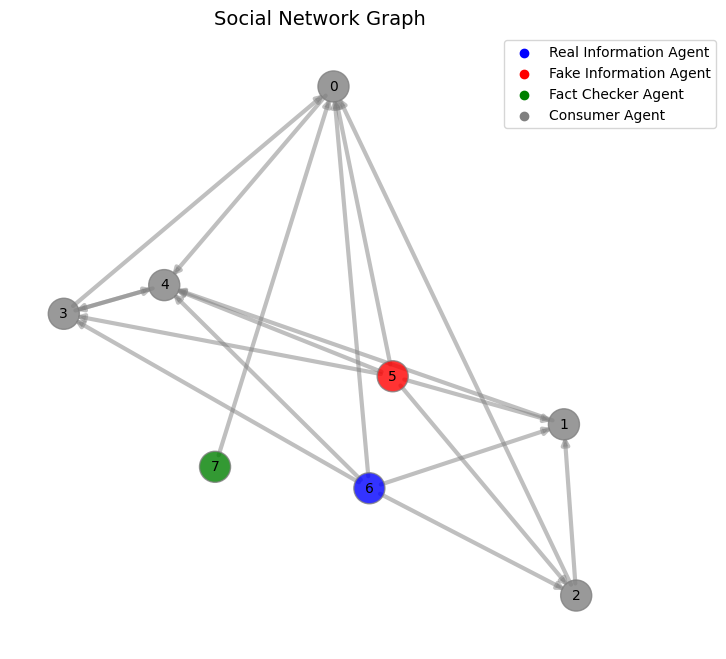
\includegraphics[width=0.5\textwidth]{../results/images/Initial_network.png}
     \caption{5 consumer network with 3 agents.}
     \label{fig: 5 consumer network, 3 agents}
 \end{figure}
 

 The initial trust levels for all consumers will be 0 and the agents will have a random action space indicating if they decide to send information to their neighbors. 

\pagebreak
\textbf{Output after the first epoch:}

\begin{verbatim}
Fake Agent: 
reward: 0, penalty : 3, influenced : None, qval : 0.0

Real Agent: 
reward: 1, penalty : 1, influenced : {4}, qval : 0.0

Fact Checker Agent: Agent type: real-information penalty: 1 reward: 1 trust level: 0.2

Fact-checker found no fake news in node Agent type: 
real-information penalty: 1 reward: 1 trust level: 0.2.

set of fake information agents audited:  None
Consumer trust level before fact checking  [0.0, -0.1, -0.1, 0.1, -0.2, 0.0, 0.0, 0.0]
Consumer trust level after fact checking [0.0, -0.1, -0.1, 0.1, -0.2, 0.0, 0.0, 0.0]

\end{verbatim}

We can see that after our first epoch, the fake-information agent has already accrued a penalty of 3 and the real agent has accrued a reward of 1 and a penalty of 1. These reward/penalties are a direct result from whether or not a consumer is accepting or denying their information. As a result, each consumers trustLevel is increasing or decreasing. At the end of the epoch, our fact checking agent kicks into gear and finds no fake information being spread across the network, and so the trust levels stand for this scenario. Because no false information was found, the consumer trust levels before and after the fact checker was introduced stay the same.

\textbf{Scenario 1: 5 consumer network at final epoch}

\begin{figure}[htbp]
     \centering
     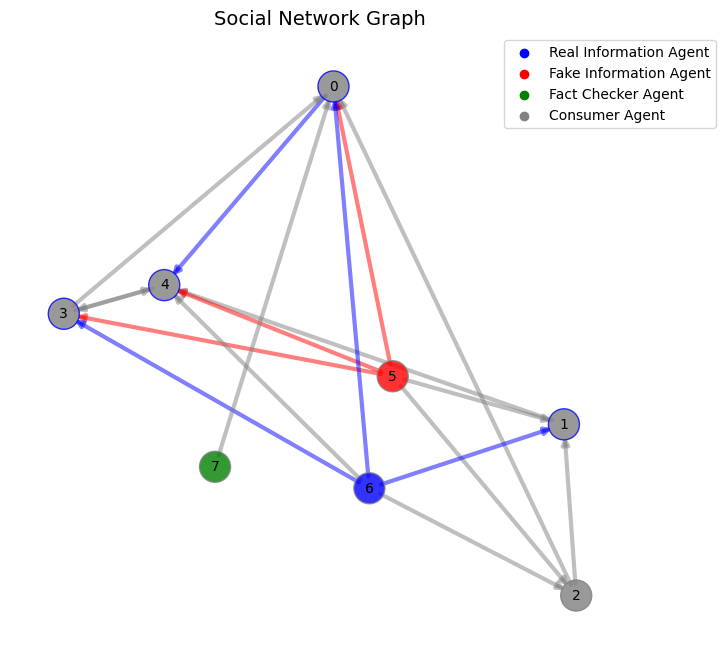
\includegraphics[width=0.5\textwidth]{../results/images/output1.png}
     \caption{5 consumers with 3 agents after final epoch.}
     \label{fig: 5 consumer, 3 agents}
 \end{figure}
 
The network now shows at epoch 7 the information traveling from consumer to consumer, indicated by the edge color to depict whether it is false, or real information being sent.

\textbf{Output after the final epoch:}
\begin{verbatim}
--------- epoch 7 ---------------------


Fake Agent: 
reward: 7, penalty : 27, influenced : None, qval : -4.0934193

Real Agent: 
reward: 26, penalty : 6, influenced : {0, 1, 2, 4}, qval : 10.440129500000001


Fact Checker Agent: Agent type: real-information penalty: 6 reward: 26 trust level: 1.0

Agent type: fake-information penalty: 27 reward: 7 trust level: 1.0

Fact-checker penalized news agent {'agentType': 'fake-information', 'qVal': -5.68407737, 
'trustLevel': 0.0, 'reward': 7, 'penalty': 27}.

set of fake information agents audited:  
{Agent type: fake-information penalty: 28 reward: 7 trust level: 1.0}

Consumer trust level before fact checking:  
[-1.1, -1.7, -1.5, -0.85, -2.1500000000000004, 0.0, 0.0, 0.0]

Consumer trust level after fact checking: 
[-1.25, -1.8499999999999999, -1.65, -1.0, -2.3000000000000003, 0.0, 0.0, 0.0]
\end{verbatim}

A few results are obvious when we analyze the outcome of this scenario from the first to the final epoch. The real-information agent ended the session with a reward of 26 and a penalty of 6. Meaning, it was able to gain more rewards opposed to penalty, successfully influencing the network. We can see that the real information agents q-value rose to 10.44. The fake information agent is opposite where it has a reward of 7, and a penalty of 27, meaning that it was not quite successful in influencing the network. The fake information agent ends the scenario with a negative q-value at -4.09 and was unable to influence the network. The penalty and negative q-value reflect the fact that the fact-checker was able to do a good job punishing this agent for not being deceptive enough. 

\begin{figure}[htbp]
     \centering
     \begin{minipage}[b]{0.45\textwidth}
         \centering
         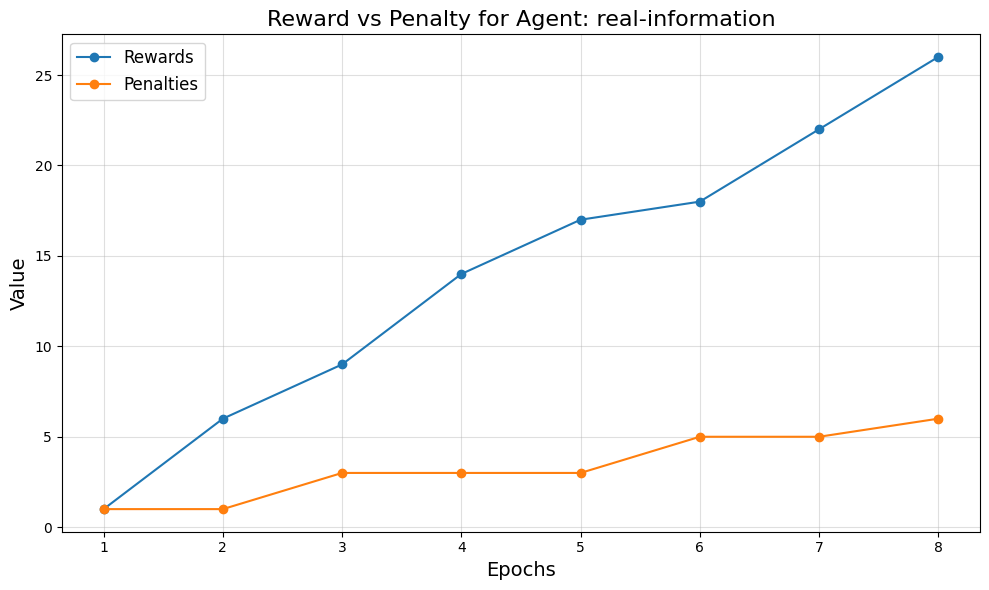
\includegraphics[width=\textwidth]{../results/images/real_info_rp.png}
         \caption{Real info Agent reward vs penalty}
         \label{fig:image1}
     \end{minipage}
     \hfill
     \begin{minipage}[b]{0.45\textwidth}
         \centering
         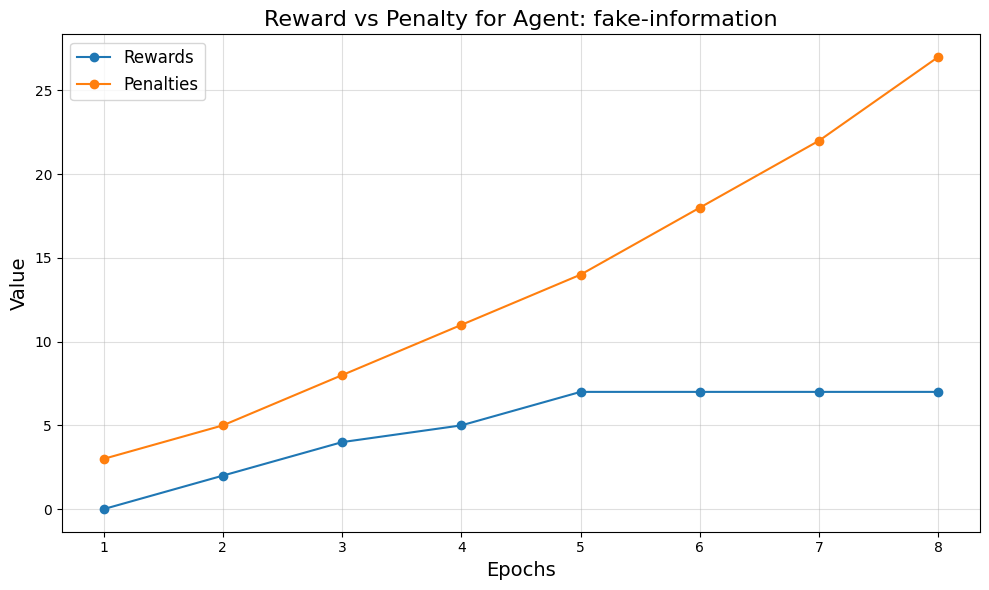
\includegraphics[width=\textwidth]{../results/images/fake_info_rp.png}
         \caption{Fake info Agent reward vs penalty}
         \label{fig:image2}
     \end{minipage}
 \end{figure}
 


Lastly, consumers trust significantly decreased. While the spread of real information was apparent, the fact that the fake information spreader has such a high penalty indicates it was caught various times throughout our simulation and therefore consumer trust ended negative, infact here are some visuals to see it:

\begin{figure}[htbp]
     \centering
     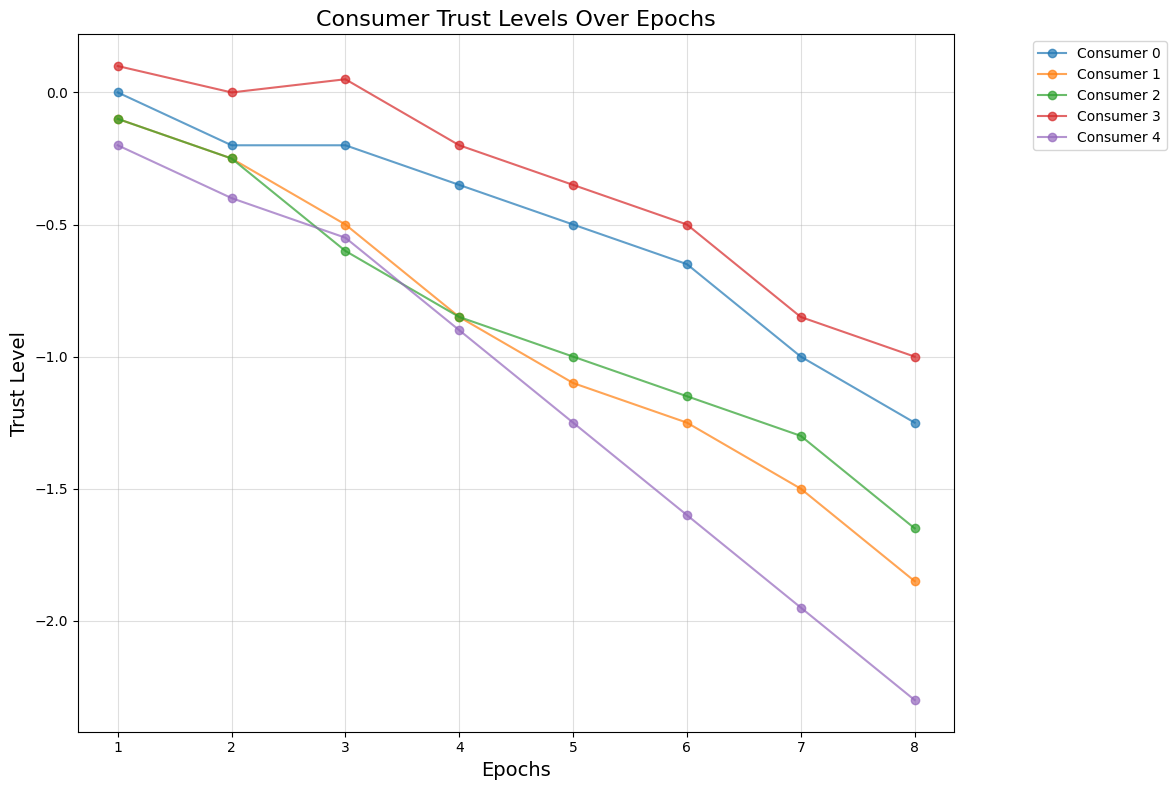
\includegraphics[width=0.5\textwidth]{../results/images/consumertrust.png}
     \caption{Consumer Trust at end of all epochs}
     \label{fig: 52 consumer, 3 agents}
 \end{figure}

\textbf{note:} For the full set of outputs, please refer to the output.txt file inside the results folder for the specific number of consumer network you want to analyze. This is shortened for the report to reduce the number of images and output text necessary.

\section{Conclusions}

\section{Individual Tasks}

\section{References}
[1] M. Goindani and J. Neville, "Social Reinforcement Learning to Combat Fake News Spread," *Proceedings of Machine Learning Research*, vol. 115, pp. 1–15, 2020.



%\input{policies.tex}

\end{document}
